% $Header$

\documentclass{beamer}

% This file is a solution template for:

% - Giving a talk on some subject.
% - The talk is between 15min and 45min long.
% - Style is ornate.



% Copyright 2004 by Till Tantau <tantau@users.sourceforge.net>.
%
% In principle, this file can be redistributed and/or modified under
% the terms of the GNU Public License, version 2.
%
% However, this file is supposed to be a template to be modified
% for your own needs. For this reason, if you use this file as a
% template and not specifically distribute it as part of a another
% package/program, I grant the extra permission to freely copy and
% modify this file as you see fit and even to delete this copyright
% notice. 


\usetheme{metropolis}



\usepackage[english]{babel}
\usepackage[english]{isodate}
\usepackage{datetime}
\usepackage{pdfpc-commands}
\usepackage{pdfpcnotes}
% or whatever

\usepackage[latin1]{inputenc}
% or whatever

% Or whatever. Note that the encoding and the font should match. If T1
% does not look nice, try deleting the line with the fontenc.


\title[Gap year internship] % (optional, use only with long paper titles)
{A Year in Industry in your gap year}

%\subtitle
%{Presentation Subtitle} % (optional)

\author[Author] % (optional, use only with lots of authors)
{T.~Eaton\inst{1}} 
% - Use the \inst{?} command only if the authors have different
%   affiliation.

\institute[Company] % (optional, but mostly needed)
{
  \inst{1}%
  Aerospace Engineering department\\
  LiveLink Technology
  \pnote{Introduce myself}
  \pnote{Old KES student}
  \pnote{Left last year}
  \pnote{Maths physics computer science A level}
% - Use the \inst command only if there are several affiliations.
% - Keep it simple, no one is interested in your street address.
}

\date[KES Presentation] % (optional)
{\formatdate{13}{11}{2017}}

\subject{Talks}





% If you wish to uncover everything in a step-wise fashion, uncomment
% the following command: 

%\beamerdefaultoverlayspecification{<+->}


\begin{document}

\selectlanguage{english}

\begin{frame}
  \titlepage
\end{frame}

\begin{frame}{Outline}
  \tableofcontents
  % You might wish to add the option [pausesections]
  \pnote{Going to talk about YINI and how to get onto the scheme}
  \pnote{What I am doing for my YINI}
\end{frame}


% Since this a solution template for a generic talk, very little can
% be said about how it should be structured. However, the talk length
% of between 15min and 45min and the theme suggest that you stick to
% the following rules:  

% - Exactly two or three sections (other than the summary).
% - At *most* three subsections per section.
% - Talk about 30s to 2min per frame. So there should be between about
%   15 and 30 frames, all told.

\section{Year in Industry}


\begin{frame}{What is Year in Industry?}
  % - A title should summarize the slide in an understandable fashion
  %   for anyone how does not follow everything on the slide itself.

  \begin{itemize}
  \item
	  Scheme run by the EDT
	  \pnote{Engineering development trust, helps create links between good students and employers}
  \item
	  Organises year long placements
	  \pnote{Can be more or less, but standard is 1 yr}
  \item
	  For pre-uni and undergrad students
	  \pnote{I will talk about pre uni application}
  \end{itemize}
\end{frame}

\begin{frame}{How does it work?}
	\begin{itemize}
		\item
			Complete online application form
		\item
			Send C.V to YINI
		\item 
			Interview with YINI
		\item
			Interview with company
			\pnote{Have to go to company in most cases}
		\item
			Year long placement
 	\end{itemize}
\end{frame}



\begin{frame}{Application process}
	Online form
	\begin{itemize}
		\item
			10-15 minutes
			\pnote{This is for first attempt. They send it back to you and recommend improvents. Iterative process"}
		\item
			Exam results
			\pnote{Have to include predicted grades aswell}
		\item
			A bit about you	
		\pnote{Hobbies, career goals etc}
	\end{itemize}
\end{frame}

\begin{frame}{Application process}
	C.V
	\begin{itemize}
		\item
			Exam results
		\item
			What you want to do in year
			\pnote{Make sure you're specific or will be miserable year}
		\item 
			Why you should be employe
			\pnote{Really sell yourself. Can ask careers advisor for help with cv}
	\end{itemize}
\end{frame}

\begin{frame}{Interviews}
	\begin{itemize}
		\item
			Telephone interview with YINI
			\pnote{Around 15 mins. Similar questions to CV. They will  score you after interview and tell you how to improve}
		\item 
			Interview with company
			\pnote{Varies greatly between companies. Will ask more about things you said in CV, so make sure you don't lie}
	\end{itemize}
\end{frame}

\section{My placement}
\begin{frame}{LiveLink Technology}
	\begin{itemize}
		\item
			Technology company in Havant
			\pnote{Mainly photokiosks and web software}
		\item
			Started August 1
			\pnote{Starting date organised with company}
		\item
			Working on BMS for quadcopters
			\pnote{Battery management system}
	\end{itemize}
\end{frame}

\begin{frame}{BMS}
	LiPo batteries are dangerous!
	\centering
	\inlineMovie{lipo.mp4}{lipo.png}{height=0.7\textheight}
	\pnote{Extreme energy density. Great for powering but very dangerous}
\end{frame}

\begin{frame}{BMS}
	System I designed
	\begin{itemize}
		\item
			Records cell voltages
		\item
			Temperature of critical points
		\item 
			Current reading
		\item 
			All sent back to control
	\end{itemize}
\end{frame}

\begin{frame}{BMS}
        \centering
        PCB I designed\\ 
        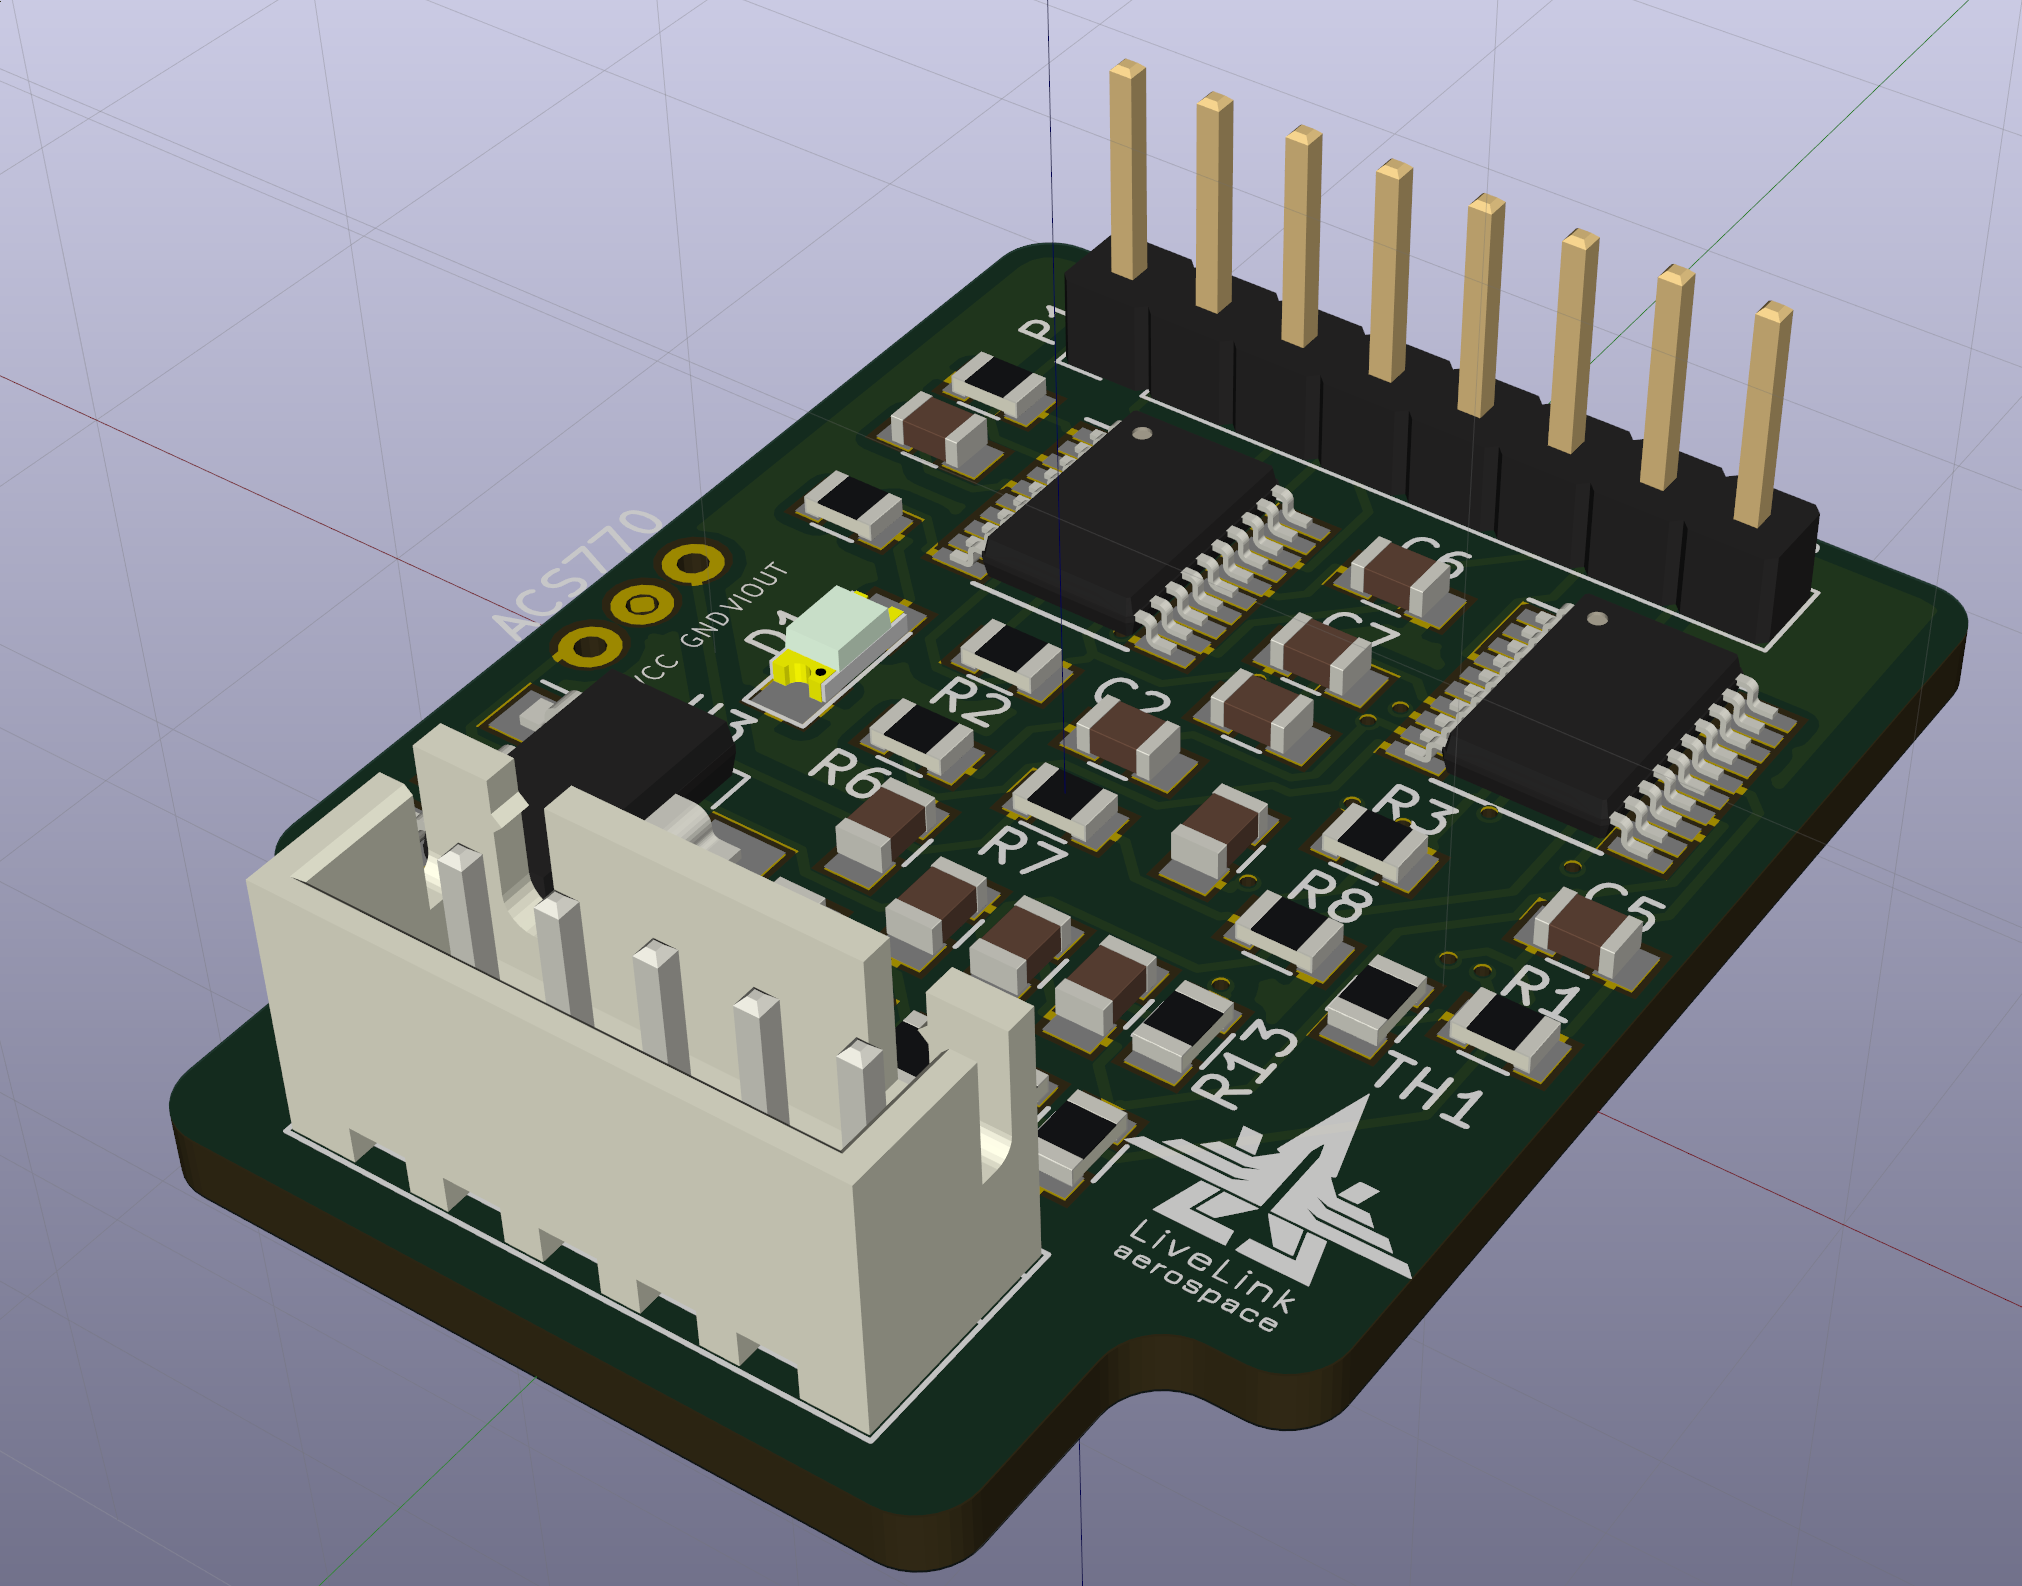
\includegraphics[scale=.1]{pcb.png}
\end{frame}

\section*{Summary}

\begin{frame}{Summary}

  % Keep the summary *very short*.
  \begin{itemize}
  \item
	  \alert{YINI} is a great way to spend gap year productively
  \item
	  Can apply easily online
  \item
	  Apply as early as possible
  \end{itemize}
\end{frame}

\begin{frame}{Contact me}
    \begin{itemize}
        \item Email: \url{t.eaton@livelinktechnology.net}
        \item
            Website: \url{tomeaton.uk}
    \end{itemize}
\end{frame} 

\end{document}

